\documentclass[border=10pt]{standalone}

\usepackage{tikz}
\usepackage{tikzsymbols}
\usetikzlibrary{calc,patterns,shapes.geometric}

\def\centerarc[#1](#2)(#3:#4:#5){\draw[#1] ($(#2)+({#5*cos(#3)},{#5*sin(#3)})$) arc (#3:#4:#5);}

\begin{document}
	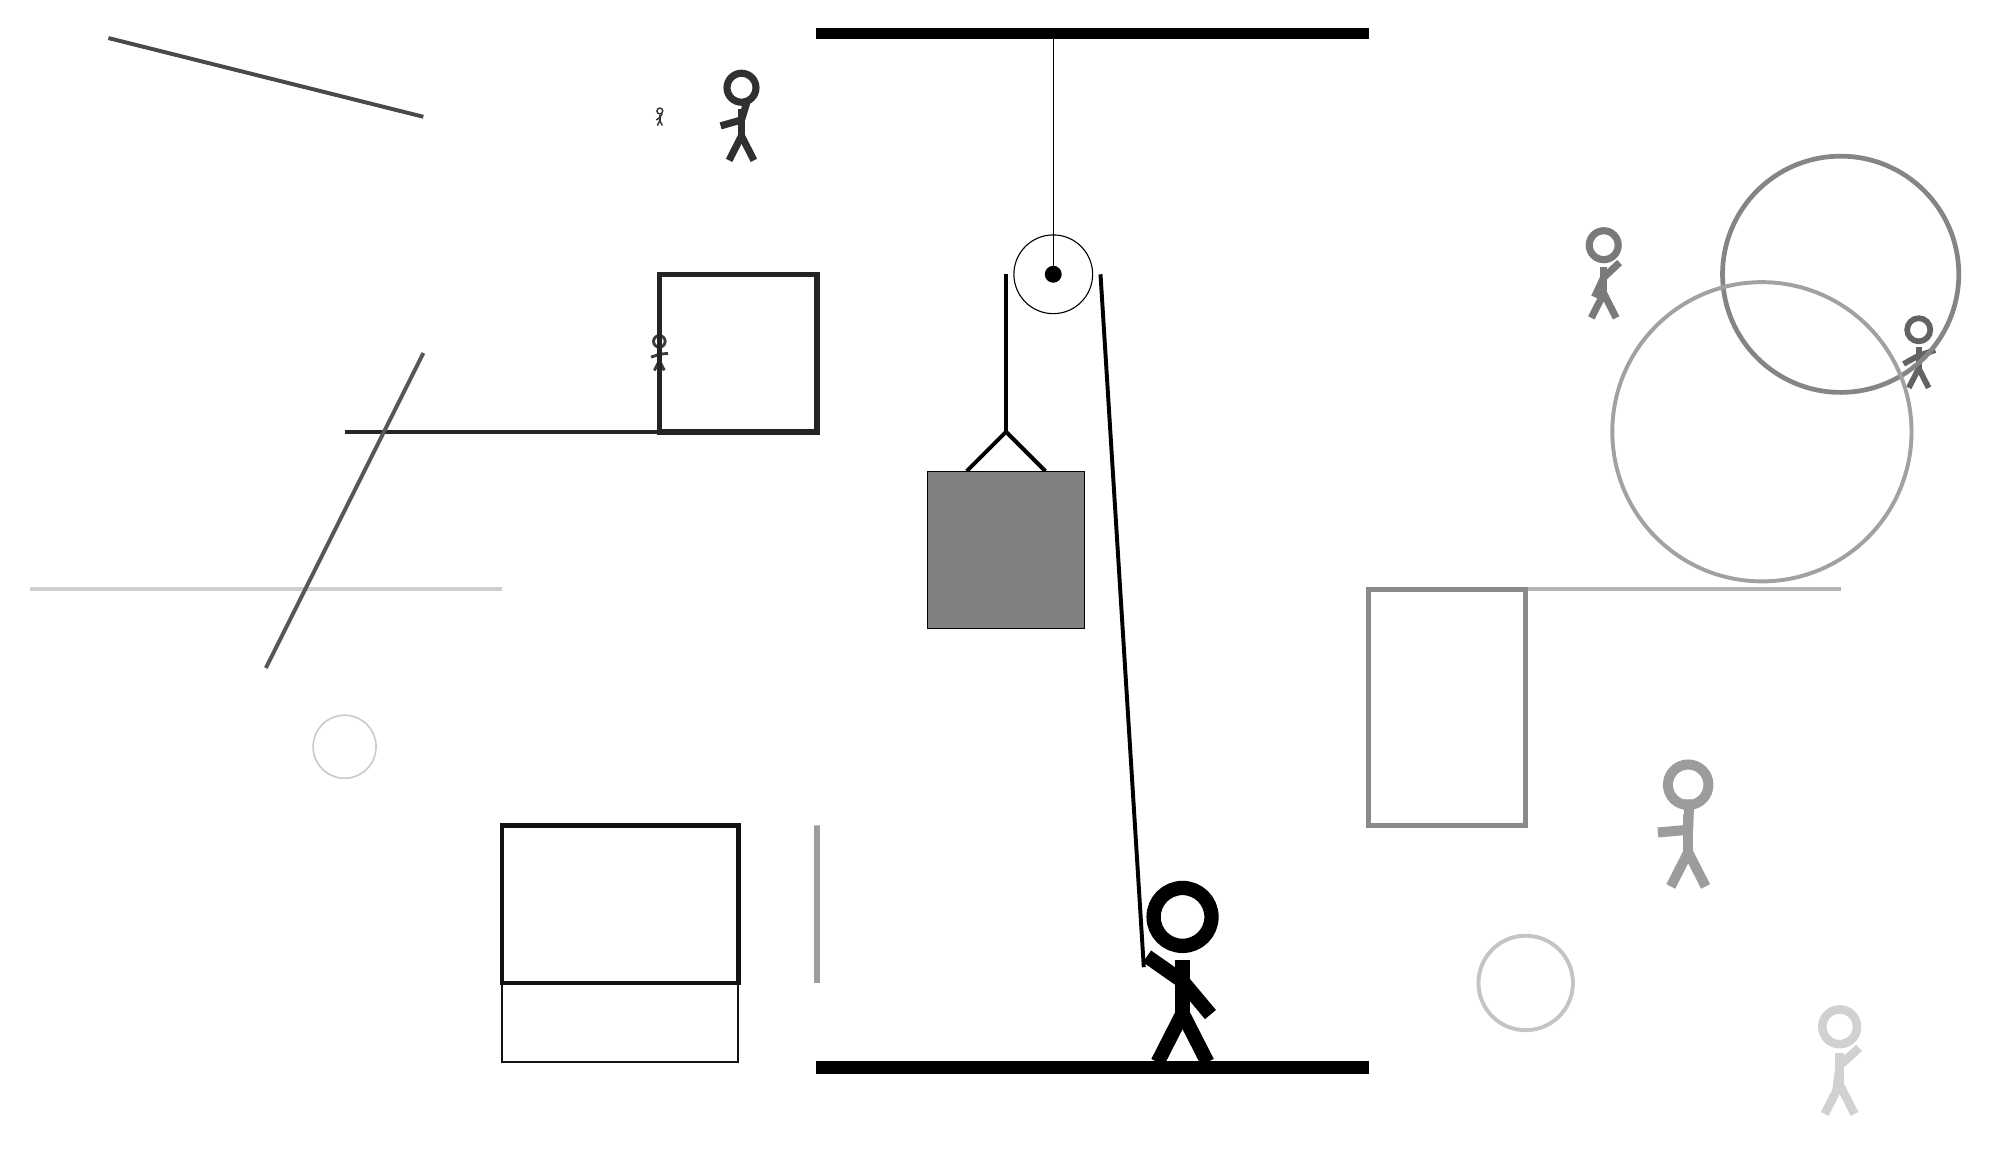
\begin{tikzpicture}
		%%%%% START %%%%%
		
		\draw[fill=black] (-2, 10) rectangle (5, 10.125);
		
		\draw (1, 7) circle (0.5);
		\draw[fill=black] (1, 7) circle (0.1);
		\draw (1, 10) -- (1, 7);
		
		\node[line width=0.6mm, color=black!81] at (-3, 9) {\Strichmaxerl[5][16][73]};
		
		\node[line width=0.2mm, color=black!39] at (9, 0) {\Strichmaxerl[7][5][88]};
		\draw[line width=0.5mm, color=black!19](-6, 3) -- (-12, 3);
		\draw[line width=0.6mm, color=black!93] (-3, 0) rectangle (-6, -2);
		\draw [line width=0.5mm, color=black!23](7, -2) circle (0.6);
		
		\node[line width=0.6mm, color=black!77] at (-4, 6) {\Strichmaxerl[2][19][6]};
		\node[line width=0.5mm, color=black!61] at (12, 6) {\Strichmaxerl[4][29][18]};
		\draw[line width=0.5mm, color=black!71](-7, 9) -- (-11, 10);
		\draw [line width=0.4mm, color=black!33](12, 1) circle (0.0);
		\draw[line width=0.5mm, color=black!29](5, 3) -- (11, 3);
		\node[line width=0.4mm, color=black!18] at (11, -3) {\Strichmaxerl[6][83][42]};
		\draw[line width=0.3mm, color=black!92] (-3, -2) rectangle (-6, -3);
		\draw [line width=0.6mm, color=black!48](11, 7) circle (1.5);
		\draw [line width=0.5mm, color=black!37](10, 5) circle (1.9);
		\draw[line width=0.5mm, color=black!85](-3, 5) -- (-8, 5);
		\draw[line width=0.5mm, color=black!66](-7, 6) -- (-9, 2);
		
		\draw[line width=0.6mm, color=black!46] (5, 3) rectangle (7, 0);
		\draw[line width=0.7mm, color=black!86] (-4, 5) rectangle (-2, 7);
		\node[line width=0.4mm, color=black!81] at (-4, 9) {\Strichmaxerl[1][37][58]};
		
		\draw[line width=0.7mm, color=black!38] (-2, -2) rectangle (-2, 0);
		\draw [line width=0.2mm, color=black!21](-8, 1) circle (0.4);
		
		\node[line width=0.5mm, color=black!52] at (8, 7) {\Strichmaxerl[5][65][43]};
		
		\draw[line width=0.5mm] (-0.1, 4.5) -- (0.4, 5.0) -- (0.9, 4.5);
		\draw[fill=black!50] (-0.6, 4.5) rectangle (1.4, 2.5);
		
		\draw[line width=0.5mm] (0.4, 7) -- (0.4, 5.0);
		\centerarc[line width=0.5mm](1, 7)(0:180:0.6);
		\draw[line width=0.5mm](1.6, 7) -- (2.15, -1.8);
		
		\node at (2.6, -1.9) {\Strichmaxerl[10][-35][-50]};
		
		\draw[fill=black] (-2, -3) rectangle (5, -3.15);
		
		%%%%% END %%%%%
	\end{tikzpicture}
\end{document}